
\section{Reflectie Lesbezoek Docent VDO}
\label{sec:lesbezoek}
De les die bezocht werd viel precies binnen de periode dat ik ook bezig was met mijn leerdoel: 4x een les voorbereiden aan de hand van een lesplan. Die lessen gingen ook heel erg goed. Zelf kreeg ik het idee dat ik soms weinig \textit{witruimte} laat tijdens de les. Elk moment is ingevuld. Soms kan ik de studenten best even ruimte geven om even na te denken en zelf te besluiten wat ze gaan doen. Tijdens de les deed ik achter elkaar:
\begin{itemize}
  \item een intro op de les
  \item kahoot
  \item duo's overleggen
  \item codedemo

\end{itemize}
Achteraf gezien had ik deze beter kunnen uitsmeren over de les.

Ongeacht mijn eigen gevoel over de les, kreeg ik overwegend positieve feedback van Lia. Met de kanttekening dat ik de didactiek en het proces meer mag benoemen tijdens de les. Of een vraag zou kunnen doorspelen naar een andere student in plaats van als docent de alwetende Ivoren Toren spelen. 
Verder is de feedback positief. De dingen waar ik op kan letten neem ik mee.

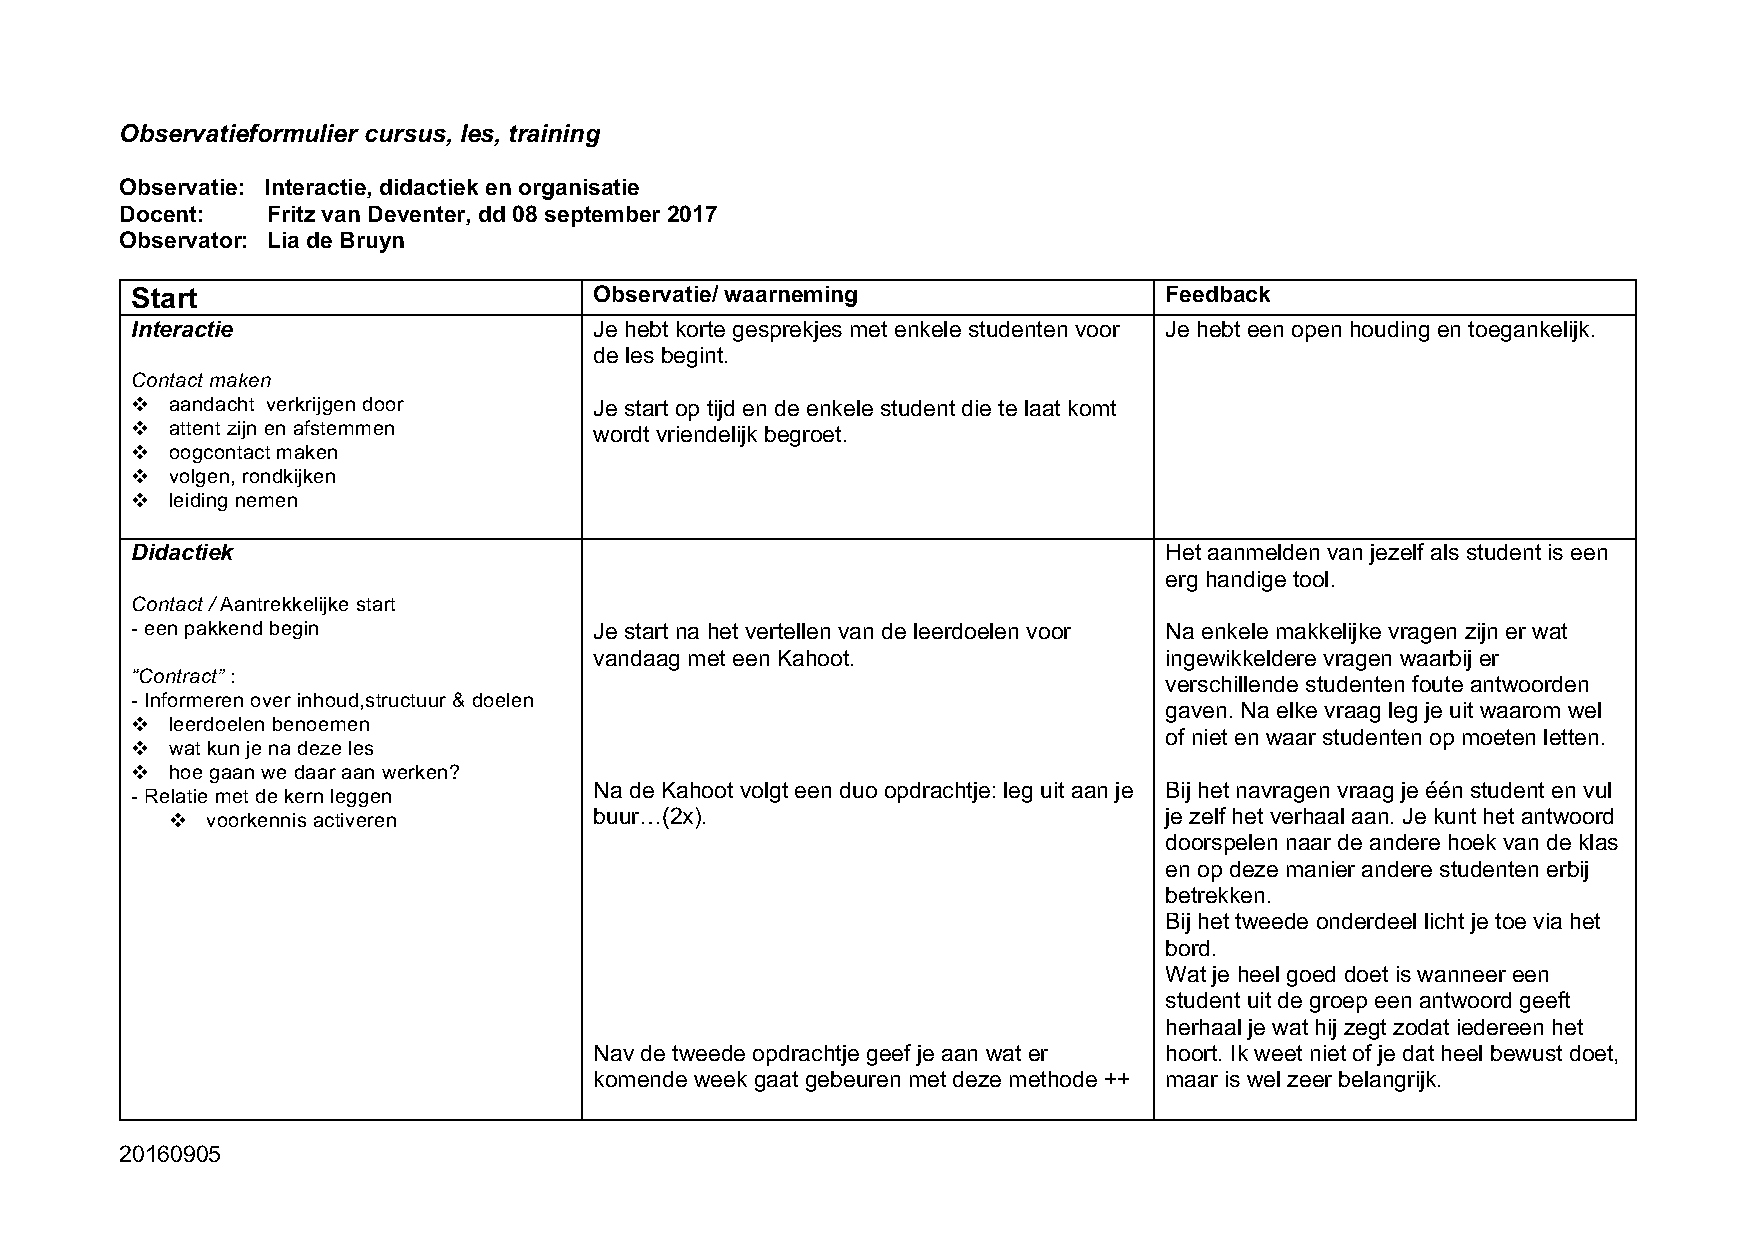
\includepdf[pages=-]{ObservatieLia.pdf}